\section{YARN"=Modell}\label{sec:yarnModel}

\begin{figure}
    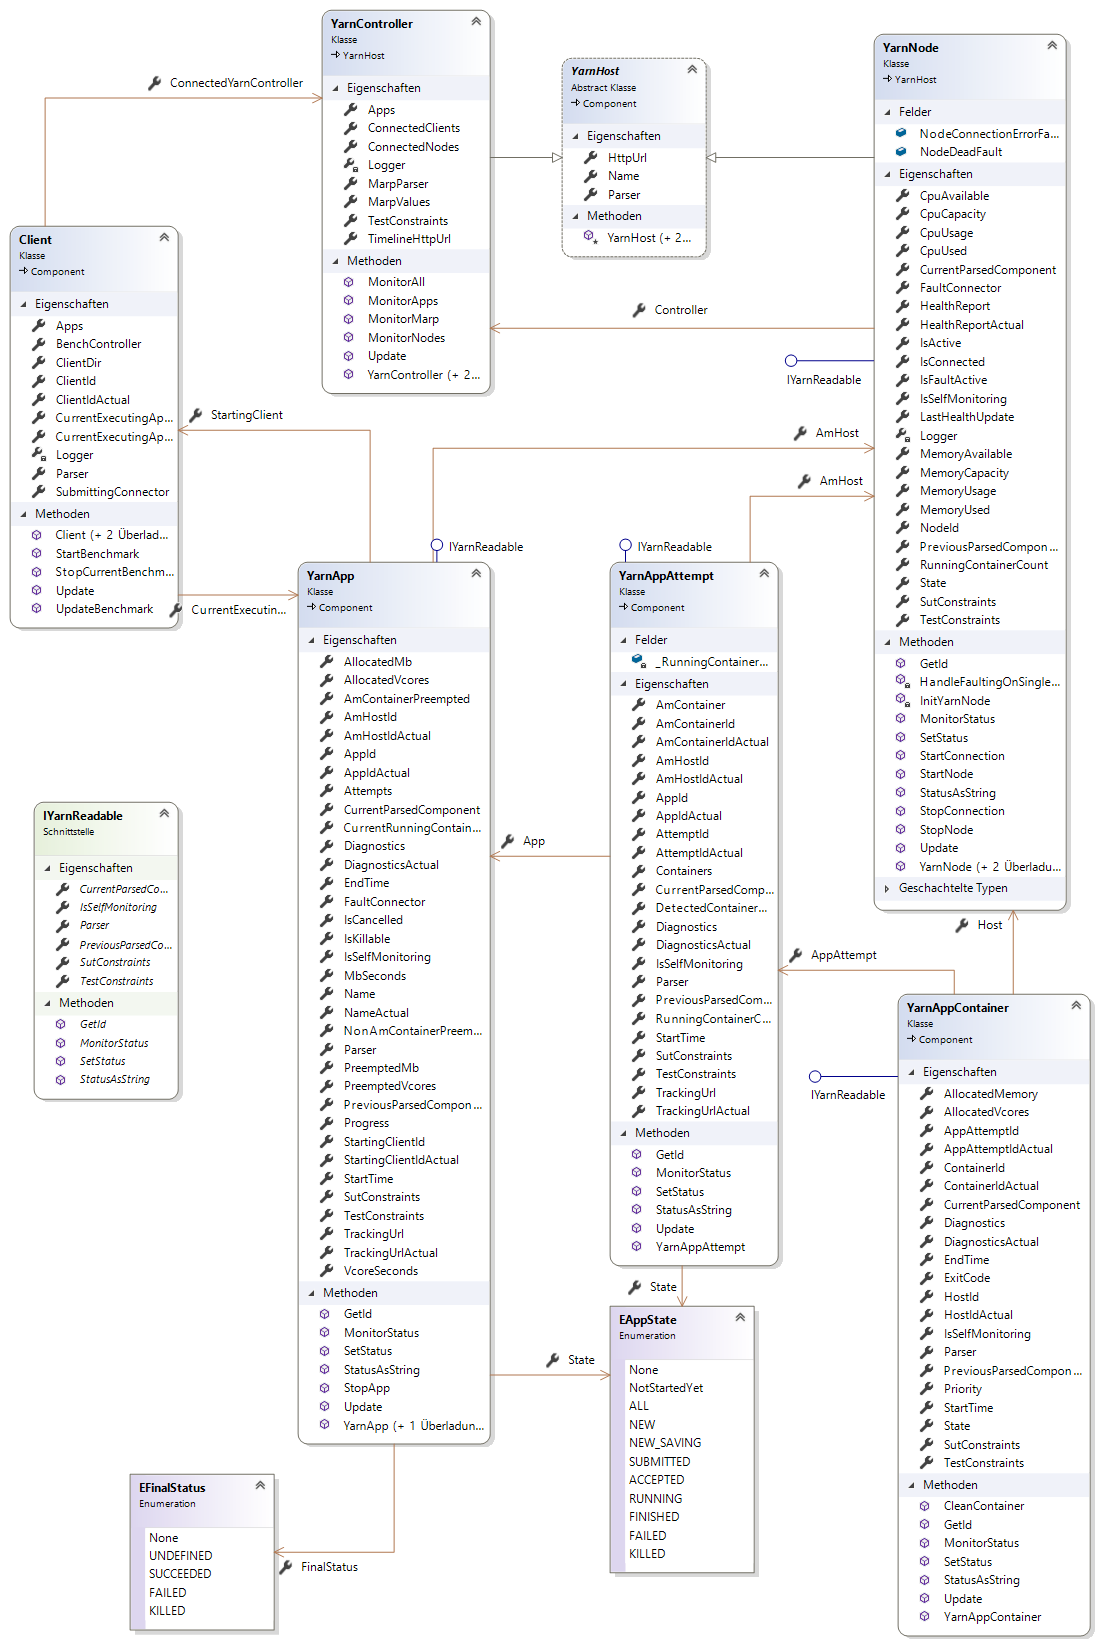
\includegraphics[width=\columnwidth]{./images/yarnModel.png}
    \caption[Aufbau des YARN"=Modells]
    {Aufbau des YARN"=Modells.
        Das Modell wurde mithilfe des Klassendiagramm"=Designers in Visual Studio 2017 visualisiert.
        Daher werden Assoziationen mit höherer Multiplizität als 1, die daher mithilfe von \texttt{List<T>} umgesetzt wurden (\zB \texttt{YarnApp.Attempts}) im Diagramm nicht als Assoziationen zwischen den Klassen angezeigt.}
    \label{fig:yarnModel}
\end{figure}

\autoref{fig:yarnModel} beschreibt im Grunde bereits das gesamte von \sS verwendete YARN"=Modell.
Enthalten sind alle hier relevanten Komponenten sowie deren Eigenschaften.
Als Eigenschaften wurden die Daten aufgenommen, welche mithilfe von Shell"=Kommandos bzw. mithilfe der REST"=API von YARN ermittelt werden können.

\subsection{Modellierte YARN"=Komponenten}\label{sec:yarnComponents}

Die abstrakte Basisklasse \texttt{YarnHost} stellt die Basis für alle Hosts des Clusters dar, also dem \texttt{YarnController} mit dem \ac{RM}, und dem \texttt{YarnNode}, was einen Node darstellt, auf dem die Anwendungen bzw. deren Container ausgeführt werden.
Die abstrakte Eigenschaft \texttt{YarnHost.HttpPort} dient als Hilfs"=Eigenschaft, da Controller und Nodes unterschiedliche Ports für die Weboberfläche nutzen, deren URL mit Port in der Eigenschaft \texttt{YarnHost.HttpUrl} abrufbar ist.
Sie wird daher vom Controller bzw. Node mit dem entsprechenden Port versehen.

Die mithilfe von \texttt{YarnApp} dargestellten Anwendungen werden mithilfe des \texttt{Bench"-Controller}s (vgl. \autoref{sec:AppImplementation}) eines Clients (entsprechend repräsentiert durch die gleichnamige Klasse) gestartet.
Jeder Client kann nur eine Anwendung ausführen, daher gibt es die Möglichkeit, mehrere Clients zum Starten von mehreren gleichzeitig ausgeführten Anwendungen zu nutzen.
Die Anwendungen selbst enthalten neben grundlegenden Daten wie \zB den Namen auch einige Daten zum Ressourcenbedarf (Speicher und CPU).
Zwar gibt Hadoop nicht direkt die zu der Anwendung gehörigen Job"=Ausführungen an, allerdings können diese mithilfe der \texttt{YarnApp.AppId} sehr einfach ermittelt werden und dann in der Liste \texttt{YarnApp.Attempts} gespeichert werden.
Das Feld \texttt{YarnApp.IsKillable} gibt an, ob die Ausführung der Anwendung mit den aktuellen Daten im Modell durch den Komponentenfehler \texttt{YarnApp.KillApp} abgebrochen werden kann.
Abhängig ist das durch \texttt{YarnApp.FinalStatus}, was angibt, ob eine Anwendung erfolgreich oder nicht erfolgreich ausgeführt wurde oder die Ausführung noch nicht abgeschlossen ist (durch \texttt{EFinalStatus.UNDEFINED}).
Um die Komponentenfehler zu aktivieren bzw. bei Bedarf auch wieder zu deaktivieren, besitzen \texttt{YarnNode} und \texttt{YarnApp} jeweils die Eigenschaft \texttt{FaultConnector}, mit der auf den benötigten Connector zugegriffen werden kann.

Jede Ausführung \texttt{YarnAppAttempt} hat eine eigene ID und kann einer Anwendung zugeordnet werden.
Genau wie bei den Anwendungen selber wird hier direkt der Node gespeichert, auf welchem der \ac{AppMstr} ausgeführt wird und einen eigenen Container bildet, dessen ID direkt gespeichert wird.
Container (dargestellt durch \texttt{YarnAppContai"-ner}) existieren in Hadoop nur während der Laufzeit eines Programmes und enthalten nur wenige Daten, darunter ihr ausführender Node.
Jede Anwendung, deren Ausführungen und deren Container enthalten zudem den derzeitigen Status, ob die Komponente noch initialisiert wird, bereits ausgeführt wird oder beendet ist.
\texttt{EAppState.NotStartedYet} dient als Status, den es nur im Modell gibt und angibt, dass die Anwendung im späteren Verlauf der Testausführung gestartet wird.

Alle vier YARN"=Kernkomponenten implementieren das Interface \texttt{IYarnReadable}, was angibt, dass die Komponente ihren Status aus Hadoop ermitteln kann.
Entsprechend wird in allen Komponenten die Methode \texttt{ReadStatus()} implementiert, in welchem mithilfe des angegebenen Parsers auf den SSH"=Treiber zugegriffen werden kann und die Komponenten im Modell so ihre eigenen Daten aus dem realen Cluster ermitteln können.
Da die REST"=API ermöglicht, alle Daten auch über die reinen Listen zu erhalten anstatt ausschließlich über die Detailausgabe, besteht auch im Modell mithilfe der Eigenschaft \texttt{IsRequireDetailsParsing} das Ermitteln der Daten so einzustellen, dass die übergeordnete YARN"=Komponente bereits alle Daten ermittelt und der Untergeordneten zum Speichern (mittels \texttt{SetStatus()}) übergibt.
Als Basis dazu dient der \texttt{YarnController}, der dafür die Daten aller Anwendungen ausliest, die wiederum die Daten ihrer Ausführungen auslesen, welche dann die Daten ihrer Container auslesen und den Komponenten zum Speichern übergeben.

\subsection{Implementierung der Komponentenfehler}\label{sec:implementedFaults}

Die Felder \texttt{YarnNode.NodeConnectionError} und \texttt{YarnNode.NodeDead} definieren die Komponentenfehler, wenn ein Node seine Netzwerkverbindung verliert bzw. beendet wird.
Die aus den Komponentenfehlern resultierenden Effekte werden in den dafür implementierten geschachtelten Klassen definiert.
\autoref{lst:faultInjection} zeigt beispielhaft die Implementierung und Injizierung des \texttt{NodeDead}"=Komponentenfehlers mithilfe des für den Node verwendeten \texttt{CmdConnector} (vgl. \autoref{sec:implementedConnectors}).
Die Injizierung des \texttt{NodeConnectionError}"=Komponentenfehlers und die Aufhebung beider Komponentenfehler sind analog implementiert.

\lstinputlisting[label=lst:faultInjection,
caption={[Injizierung eines Komponentenfehlers]
    Injizierung eines Komponentenfehlers (gekürzt).
    Sollte der Node nicht beendet werden, wird die Injizierung einmalig erneut versucht. \texttt{CmdConnector.Faulting} ist der für Komponentenfehler verwendete Connector.},
float,style=cs]
{./listings/faultInjectionExample.cs}

\subsection{Fehlerüberprüfung}\label{sec:FaultTesting}

Um zu prüfen, ob sich das reale Cluster nach der Aktivierung bzw. Deaktivierung eines Komponentenfehlers korrekt rekonfiguriert, werden \emph{Constraints} genutzt.
\todo{Verweis zu Anforderungen}
Diese richten sich nach den funktionalen Anforderungen des Systems und prüfen, ob diese weiterhin eingehalten werden.
Da die funktionalen Anforderungen bei jeder YARN"=Komponente unterschiedlich sind, wurden diese mithilfe der Eigenschaft \texttt{IYarnReadable.Constraints} für jede Komponente einzeln definiert.
